\documentclass[english,version-2020-11]{uzl-thesis}

\UzLThesisSetup{
  Masterarbeit,
  Logo-Dateiname        = {uzl-thesis-logo-itcs.pdf},
  Verfasst              = {am}{Institut für Theoretische Informatik},
  Titel auf Deutsch     = {Über elementare Eigenschaften einer mehrdimensionalen Verallgemeinerung des euklidischen Algorithmus},
  Titel auf Englisch    = {On Elementary Properties of a Multi-Dimensional Generalization of the Euclidean Algorithm},
  Autor                 = {Daniel Knaack},
  Betreuerin            = {Prof. Dr. Kim-Manuel Klein},
  Studiengang           = {Informatik},
  Datum                 = {18. Juni 2024},
  Abstract              = {TODO},
  Zusammenfassung       = {TODO},
  Numerische Bibliographie,
}

\UzLStyle{alegrya modern design}

\newcommand\Z{{\mathbb Z}}
\newcommand\Q{{\mathbb Q}}

\begin{document}

\chapter{Introduction}

\chapter{Preliminaries}

\section{Continued Fraction}

\begin{definition}
  A continued fraction for a (potentially infinite) list of numbers $a_0, a_1,
  \dots \in \Z$ is defined as
  \begin{align*}
    [a_0; a_1, \dots] = a_0 + \frac{1}{[a_1; a_2, \dots]}
  \end{align*}
\end{definition}

\begin{definition}
  The $n$-th convergent of a continued fraction $[a_0; a_1, \dots]$
  is defined as the finite continued fraction $[a_0; a_1, \dots, a_n]$.
\end{definition}

\begin{definition}
  Each convergent has a canonical structure:
  \[
    [a_0; a_1, \dots, a_n] = \frac{p_k}{q_k} = \frac{p_k(a_0, \dots, a_k)}{p_{k-1}(a_1, \dots, a_k)}.
  \]
\end{definition}

\section{Generalized Euclidean Algorithm}

\begin{Pseudocode}
while $x$ is not integral do
  solve $Bx = c$
  find $x_l$ which is not integral
  swap $B_l$ and $c$
  ...
end
\end{Pseudocode}

\begin{align*}
  x_i' = \begin{cases}
    1 / x_l, & \text{ if } i = l, \\
    x_i / x_l & \text{ otherwise.}
  \end{cases}
\end{align*}

\section{Algebraic Numbers}

\begin{definition}
  A complex number $\alpha$ is an algebraic number if $\alpha$ is the root of some monic polynomial with rational coefficients
  \[
    p(\alpha) = 0, \quad p(x) = x^n + a_{n-1} x^{n-1} + \dots a_1 x + a_0, \quad a_0, a_1, \dots, a_{n-1} \in \Q.
  \]
\end{definition}

\begin{definition}[Ring]
  A ring is a set $R$ with two binary operations $+$ (addition) and $\cdot$ (multiplication)
  satisfying the following conditions:
  \begin{enumerate}
    \item $(R, +)$ is a commutative group.
    \item $(R, \cdot)$ is a monoid, i.e. $\cdot$ is associative and there exists an identity element $1 \in R$.
    \item Multiplication is distributive with respect to addition:
      \begin{align*}
        a \cdot (b + c) = (a \cdot b) + (a \cdot c), & \quad \text{for all } a, b, c \in R \\
        (b + c) \cdot a = (b \cdot a) + (c \cdot a), & \quad \text{for all } a, b, c \in R
      \end{align*}
  \end{enumerate}
  A ring is commutative if multiplication is commutative.
\end{definition}

\begin{definition}[Ideal]
  % TODO: Add note about left and right-sided ideals?
  Given a commutative ring $R$, an ideal $I$ is a subset of $R$ satisfying
  \begin{enumerate}
    \item $(I, +)$ is a subgroup of $(R, +)$
    \item For every $r \in R$ and every $x \in I$, the $r \cdot x \in I$.
  \end{enumerate}
\end{definition}

\begin{definition}[Quotient Ring]
  For an ideal $I$ over a ring $R$, the equivalence relation $\sim$ is defined as
  \[
    a \sim b \quad \text{if and only if} \quad a - b \in I.
  \]
  % TODO: Define the equivalence class of an element.
  The set of equivalence classes is denoted by $R/I$ and forms another ring with
  \begin{align*}
    (a + I) + (b + I) = (a + b) + I. \\
    (a + I) \cdot (b + I) = (a \cdot b) + I.
  \end{align*}
\end{definition}

\begin{example}
  Let $\Q[X]$ be the ring of polynomials in the variable $X$ with only rational
  coefficients and $I = (X^2 - X - 1)$ an ideal consisting of all multiples of $X^2 - X - 1$.
  Then, the operations of the quotient ring $\Q[X]/(X^2 - X - 1)$ are
  \begin{align*}
    (a_0 + a_1 X) + (b_0 + b_1 X)
    & = (a_0 + b_0) + (a_1 + b_1) X \\
    (a_0 + a_1 X) \cdot (b_0 + b_1 X)
    & = (a_0 b_0) + (a_1 b_0 + a_0 b_1) X + (a_1 b_1) X^2 \\
    & = (a_0 b_0 + a_1 b_1) + (a_1 b_0 + a_0 b_1 + a_1 b_1) X
  \end{align*}
\end{example}

The quotient ring $\Q[X]/(X^2 + X + 1)$ can also be seen as a extension field $\Q(\alpha)$ over $Q$,
where $\alpha$ is an algebraic number satisfying for the respective polynomial.
Hence, $\Q[X]/(X^2 + X + 1)$ forms a field.

\begin{definition}[Simple Extension]
  Given an algebraic number $\alpha$ of degree $d$,
  a simple extension of the rational numbers with $\alpha$ is the set
  \[
    \Q(\alpha) = \{\sum_{i=0}^d \alpha^i q_i \mid q_i \in \Q\}.
  \]
\end{definition}

\chapter{Determinant}

\section{Generalized Fibonacci Sequence}

Dividing two consecutive Fibonacci numbers approaches the golden ratio as $n$ increases.
The golden ratio is a solution to the equation $x^2 - x - 1 = 0$.
For higher dimensions, we will encounter similar polynomial equations with higher degree.
The goal of this section is to generalize the relationship between linear
recurrences like the Fibonacci sequence with their respective golden ratio.

Since the algorithm expects $x_i$ between $0$ and $1$, we have to use $1/\phi$ instead of $\phi$.
The value $1/\phi$ is the root of another polynomial $x^2 + x - 1$, which is the reciprocal
of the polynomial $x^2 - x - 1$.

\begin{definition}
  Given a polynomial $p = \sum_{i=0}^n a_i x^n$, its \emph{reciprocal polynomial},
  denoted as $p^*$, is defined as
  \[
    p^*(x) = x^n p(x^{-1}) = a_n + a_{n-1} x + \dots + a_0 x^n.
  \]
\end{definition}

\begin{example}
  The reciprocal of the golden ratio polynomial $x^2 - x - 1$ is
  \begin{align*}
    x^2 + x - 1,
  \end{align*}
  which has a root at $\psi = 1/\phi$.
\end{example}

\begin{lemma}
  Let $p$ be a polynomial. Then, $a$ is a root of $p$ if and only if $a^{-1}$ is a root of $p^*$.
\end{lemma}

\begin{proof}
  Let $a$ be a root of $p$. It follows $p^*(a^{-1}) = a^n p(a) = a^n \cdot 0 = 0$.
  Now let $a^{-1}$ be a root of $p^*$. Then $p^*(a^{-1}) = a^n p(a) = 0$.
  By construction, $a$ cannot be zero and therefore we must have $p(a) = 0$.
\end{proof}

\begin{definition}
  A linear recurrence with coefficients~$a_0, \dots, a_d$ is an equation of the
  following form:
  \[
    F(n + 1) = a_0 F(n - d) + a_1 F(n - d + 1) + \dots + a_{d-1} F(n - 1) + a_d F(n).
  \]
\end{definition}

\begin{definition}
  Given a linear recurrence~$F$ with coefficients~$a_0, \dots, a_d$, its
  \emph{characteristic polynomial} $p_F$ is defined as
  \[
    p_F(x) = x^{d+1} - a_d x^d - a_{d-1} x^{d-1} - \dots - a_1 x - a_0.
  \]
\end{definition}

\begin{example}
  The linear recurrence which has $p_d^*(x)$ as its characteristic polynomial is:
  \begin{align*}
    F(n) = F(n - 1) + (-1)^{d+1} F(n - d) - \sum_{i=2}^{d - 1} (-1)^{i+1} 2 F(n - i).
  \end{align*}
\end{example}

% TODO: Show that this converges! We're still missing the convergence criteria
\begin{lemma}
  Let $F$ be a linear recurrence with coefficients $a_0, \dots, a_d$.
  If its characteristic polynomial has a real positive root $\phi$
  and the sequence $F(n+1)/F(n)$ is converging, then
  \[
    \lim_{n \to \infty} \frac{F(n + 1)}{F(n)} = \phi.
  \]
\end{lemma}

\begin{proof}
  By assumption, the ratios approach some limit $L$. It follows:
  \[
    L
    = \lim_{n \to \infty} \frac{F(n + 1)}{F(n)}
    = \lim_{n \to \infty} a_0 + \sum_{i = 1}^d \frac{a_i F(n - d + i)}{F(n)}
  \]
  Each term in the sum can be rewritten as a product of consecutive terms:
  \[
    \frac{F(n - 1 - d + i)}{F(n - 1)}
    = \frac{F(n - 1 - d + i)}{F(n - d + i)} \frac{F(n - d + i)}{F(n - d + i + 1)} \dots \frac{F(n - 2)}{F(n-1)}.
  \]
  Hence, each term in the sum approaches $L^{-i}$,
  which results in the following polynomial:
  \[
    L = a_0 + \sum_{i = 1}^d a_{d - i} L^{-i},
    \quad \text{or equivalently} \quad
    L^{d+1} = a_0 + a_1 L + \dots + a_d L^d,
  \]
  which directly corresponds to a root of its characteristic polynomial.
\end{proof}

\begin{corollary}
  Under the same conditions, $\lim_{n \to \infty} F(n + i) / F(n) = \phi^i$ for $i > 1$.
\end{corollary}

Given, the linear recurrence $F(n + d + 1) = F(n) + a_1 F(n - 1) + \dots + a_d F(n + d)$,
the value for $x_i^{(n)}$ in the solution $x^{(n)}$ is
\begin{equation}
  \label{eq:general-solution}
  x_i^{(n)} = \frac{F(n - i) + \sum_{k=1}^{i-1} a_{d-k} F(n - k)}{F(n)}.
\end{equation}

\begin{lemma}
  Pivoting with the first element of $x^{(n)}$ using the modified update rule yields the vector
  \[
    x' = (x^{(n-1)}_2, x^{(n-1)}_3, \dots, x^{(n-1)}_d, x^{(n-1)}_1).
  \]
\end{lemma}

\begin{proof}
  For $x_1$, we get
  \[
    \begin{aligned}
      \frac{1}{x_1}
      & = \frac{F(n)}{F(n - 1)} \\
      & = a_d + \frac{F(n - d - 1) + a_1 F(n - d - 2) + \dots + a_{d-1} F(n - 2)}{F(n - 1)} \\
      & = a_d + x^{(n-1)}_d.
    \end{aligned}
  \]
  For the other values, we get
  \begin{align*}
    \frac{x_i}{x_1}
    & = \frac{F(n - i) + \sum_{k=1}^{i-1} a_{d-k} F(n - k)}{F(n)} \frac{F(n)}{F(n - 1)} \\
    & = a_{d-1} + \frac{F(n - i) + \sum_{k=2}^{i-1} a_{d-k} F(n - k)}{F(n-1)} \\
    & = x^{(n-1)}_{i+1} \qedhere
  \end{align*}
\end{proof}

\begin{corollary}
  Running the generalized Euclidean algorithm with $x^{(n)}$ as the solution to
  the linear system $B x = c$ requires $n$ steps, if $x^{(n)}_1$ is the
  smallest element in $x^{(n)}$.
\end{corollary}

Of course, the Euclidean algorithm receives a matrix $B \in \Z^{d \times d}$
and vector $c \in \Z^d$ as its input and not the solution $x$ itself.
However, we can construct a very simple linear system $B^{(n)} x = c^{(n)}$,
where $x^{(n)}$ is the solution, in the following way:
\[
  B^{(n)} =
  \begin{pmatrix}
    F(n) & 0 & \dots & 0 & 0 \\
    0 & F(n) & \dots & 0 & 0 \\
    \vdots & \vdots & \ddots & \vdots & \vdots \\
    0 & 0 & \dots & F(n) & 0 \\
    0 & 0 & \dots & 0 & F(n) \\
  \end{pmatrix},
\]
\[
  c^{(n)} =
  \begin{pmatrix}
    F(n - 1) \\
    F(n - 2) + a_{d-1} F(n - 1) \\
    \vdots \\
    F(n - d + 1) + \sum_{k=1}^{d-2} a_{d-k} F(n - k) \\
    F(n - d) + \sum_{k=1}^{d-1} a_{d-k} F(n - k) \\
  \end{pmatrix}.
\]

\begin{lemma}
  The vector $x^{(n)}$ from Equation~\ref{eq:general-solution} is a solution to the
  linear system $B^{(n)} x = c^{(n)}$.
\end{lemma}

\begin{proof}
  Follows directly from the definition of $x^{(n)}$.
\end{proof}

\section{Pivoting the Same Element}

In one dimension, a solution is bad when the value $x_1$ is close to $1$.
However, in the next iteration $x_1$ would be close to $0$ and therefore
would lead to a greater decrease in the determinant.
An initial guess would be that the solution lies exactly between $0$ and $1$ at $1/2$.
However, this solution is also good as after just one step we have achieved integrality.

The solution is to choose a value $x_1$ such that its value in the first
iteration is the same as its value in the second iteration.
This means we are trying to solve the following equation:
\[
  x_1 = 1/x_1 - 1.
\]
This gives us the polynomial $x^2 + x - 1$ where the root is the inverse of the
golden ratio.

% TODO: Explore other strategies. Can we generalize this to every possible strategy?
In just two dimensions, we already have an additional degree of freedom.
Since the solution $x$ consists of two values, we can choose which index we pivot with.
We will choose the value with the smallest fractional value as this decreases
the determinant the fastest.
We assume w.l.o.g. that our values are sorted in increasing order.
This means we pivot with $x_1$ first.

% TODO: What about just choosing the golden ratio for every x_i?
% TODO: Are odd dimensions easier since the decrease is not worse? We could
% choose two values to be the same, since the ratio for odd dimensions is
% smaller than the previous dimension
Just like in one dimension we want to choose $x_1$ carefully such that the
determinant decreases the same amount in every iteration.
A simple solution would be to fill both values with the golden ratio.
In this case, it does not matter which index we choose as each one decreases
the determinant the same amount.
However, in two dimensions we can make this decrease slightly worse
by choosing different values for $x_1$ and $x_2$ such that we swap the pivot
in each iteration.

Assuming the value for $x_1$ is already chosen where would $x_2$ be placed?
Ideally, it would be close to the right side of $x_1$, because then the new
value $-x_2 / x_1$ would be close to $-1$ and the fractional value would be
close to $1$.
Since the decrease must stay the same in each iteration, this gives us the
following two equations:
\begin{align*}
  x_1 = 2 - x_2 / x_1 \\
  x_2 = 1 / x_1 - 1,\\
\end{align*}
which leads to the following polynomial:
\begin{align*}
  x_1^3 - 2x_1^2 - x_1 + 1 = 0
\end{align*}

Let $\phi_2$ be the root of this polynomial.
If we choose $x_1 = \phi_2$ and $x_2 = 2\phi_2 - \phi_2^2$,
then the values in the second iteration are
\[\begin{aligned}
  x_1' & = 1 / x_1 - 1   &  & = 1 / \phi_2 - 1                    &  & = 2\phi_2 + \phi_2^2 &  & = x_2, \\
  x_2' & = 2 - x_2 / x_1 &  & = 2 - (2\phi_2 + \phi_2^2) / \phi_2 &  & = \phi_2             &  & = x_1
\end{aligned}\]

We can extend this to $d$ dimensions using the following equations:
\begin{align*}
  x_1 = 2 - x_2 / x_1 \\
  x_2 = 2 - x_3 / x_1 \\
  x_3 = 2 - x_4 / x_1 \\
  \vdots \\
  x_{d-1} = 2 - x_d / x_1 \\
  x_d = 1 / x_1 - 1 \\
\end{align*}

These leads us to two polynomials depending on the dimension.
\begin{itemize}
  \item For even $d$: $x - 1 + 2 x^2 - 2 x^3 + \dots + x^{d+1}$
  \item For odd $d$: $1 - x - 2 x^2 + 2 x^3 - 2 x^4 \dots + x^{d+1}$
\end{itemize}
or in one equation $p_d(x) := 1 - x - (-x)^{d+1} - \sum_{i = 2}^{d} 2 (-x)^{i} = 0$.
Let $\phi_d$ be the root of this polynomial.
Then, we choose as our solution $x = (x_1, \dots, x_d)$ with
\begin{equation}
  \label{eq:rotate-solution}
  x_1 = \phi_d, \quad x_i = 2 - x_1 x_{i-1} = -(-\phi_d)^i + \sum_{k=0}^{i-1} 2 (-\phi_d)^i.
\end{equation}

\begin{example}
  For $d = 5$, we get the following values:

  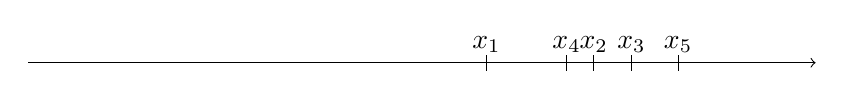
\begin{tikzpicture}[scale=10]
    \draw (0.5820216424559055, -0.01) -- node[above] {$x_1$} (0.5820216424559055, 0.01);
    \draw (0.7181491667223714, -0.01) -- node[above] {$x_2$} (0.7181491667223714, 0.01);
    \draw (0.7661126076135922, -0.01) -- node[above] {$x_3$} (0.7661126076135922, 0.01);
    \draw (0.6837042616132034, -0.01) -- node[above] {$x_4$} (0.6837042616132034, 0.01);
    \draw (0.8252940926247403, -0.01) -- node[above] {$x_5$} (0.8252940926247403, 0.01);
    \draw[->] (0, 0) -- (1, 0);
  \end{tikzpicture}
\end{example}

\begin{itemize}
  \item \textbf{Polynomial}:
    \[
      1 - x - (-x)^{d+1} - \sum_{i = 2}^{d} 2 (-x)^{i} = 0.
    \]
  \item \textbf{Algebraic Solution Vector}:
    \[
      x_i = 2x + (-x)^{i+1} + \sum_{k=2}^{i} (-x)^{k}.
    \]
  \item \textbf{Linear Recurrence}:
    \[
      F(n) = F(n - 1) + (-1)^{d+1} F(n - d) - \sum_{i=2}^{d - 1} (-1)^{i+1} 2 F(n - i).
    \]
  \item \textbf{Rational Solution Vector}:
    \[
      x_1 = \frac{F(n - 1)}{F(n)}, x_i = \frac{2 F(n-1) + (-1)^{i+1} F(n - i) + \sum_{k=2}^i (-1)^k F(n-k)}{F(n)}.
    \]
  \item \textbf{Matrix}:
    \[\left(\begin{array}{cccc|c}
      F(n)   & 0      & \dots  & 0      & F(n - 1) \\
        0    & F(n)   & \dots  & 0      & 2 F(n - 1) - F(n - 2) \\
      \vdots & \vdots & \ddots & \vdots & \vdots   \\
        0    & 0      & \dots  & F(n)   & 2 F(n-1) + (-1)^{d+1} F(n - d) + \sum_{k=2}^d (-1)^k F(n-k) \\
    \end{array}\right)\]
\end{itemize}

\begin{example}
  \begin{align*}
    \left\{ \frac{1}{x_1} \right\}
    & = \left\{ \frac{F(n - 1) + 2 F(n - 2) - 2 F(n - 3) + F(n - 4)}{F(n - 1)} \right\} \\
    & = \frac{2 F(n - 2) - 2 F(n - 3) + F(n - 4)}{F(n - 1)} \\
    \left\{ -\frac{x_2}{x_1} \right\}
    & = \left\{ -\frac{2 F(n - 1) - F(n - 2)}{F(n)} \frac{F(n)}{F(n - 1)} \right\} \\
    & = \frac{F(n - 2)}{F(n - 1)} \\
    \left\{ -\frac{x_3}{x_1} \right\}
    & = \left\{ -\frac{2 F(n - 1) - 2 F(n - 2) + F(n - 3)}{F(n)} \frac{F(n)}{F(n - 1)} \right\} \\
    & = \frac{2 F(n - 2) - F(n - 3)}{F(n - 1)}
  \end{align*}
\end{example}

\section{$d$-bonacci Numbers}

\section{Keeping Equal Distances between Neighbors}

\[
  x_1 = \frac{x_2}{x_1} - 1 = \frac{x_3}{x_2} - 1 = \dots = \frac{x_d}{x_{d-1}} = \frac{1}{x_d} - 1.
\]

\begin{itemize}
  \item \textbf{Polynomial}: \[x^{d+1} + x - 1 = 0.\]
  \item \textbf{Algebraic Solution Vector}: \[x_i = \psi^{d+1-i}.\]
  \item \textbf{Linear Recurrence}: \[F(n + 1) = F(n) + F(n - d).\]
  \item \textbf{Rational Solution Vector}: \[x_i = \frac{F(n)}{F(n-d+i)}.\]
  \item \textbf{Matrix}:
    \[\left(\begin{array}{cccc|c}
      F(n)   & 0      & \dots  & 0      & F(n - d) \\
        0    & F(n)   & \dots  & 0      & F(n - d + 1) \\
      \vdots & \vdots & \ddots & \vdots & \vdots   \\
        0    & 0      & \dots  & F(n)   & F(n - 1) \\
    \end{array}\right)\]
\end{itemize}

The algebraic solution falls apart after two iterations when pivoting with the
smallest element, i.e. $x_1$.

\section{Jacobi-Perron Algorithm}

The algorithm in this form, where we always choose the same pivot,
is equivalent to the Jacobi-Perron algorithm, which was first proposed
by Jacobi \cite{Jacobi68} and later analyzed by Perron \cite{Perron07}.
In modern times, the algorithm was picked up again by Bernstein \cite{Bernstein06}.
Each of them has analyzed the algorithm in the context of Hermite's Problem.

Charles Hermite initially posed a question to Jacobi, whether there exists a
representation of the real numbers as an infinite sequence of natural numbers
such that the sequence is eventually periodic if and only if the number is a
cubic irrational. The question remains unanswered with the latest attempt
\cite{Murru15} showing that there is an infinite sequence which is eventually
periodic for every cubic irrational.

\section{An Idempotent Solution for Two Dimensions}

Let $\vec x = (\psi, 1 - \psi)$, where $\psi$ is the only real positive root of $x^2 + x - 1$.
For this solution, it does not matter which element we choose to pivot with, it will always
yield the same result.

Pivoting with $x_1$:
\begin{align*}
  \frac{1}{x_1} - 1 & = \frac{1}{\psi} - 1 = \psi, \\
  1 - \frac{x_2}{x_1} & = 1 - \frac{1 - \psi}{\psi} = 1 - \psi.
\end{align*}

Pivoting with $x_2$:
\begin{align*}
  \frac{1}{x_2} - 2 & = \frac{1}{1 - \psi} - 2 = \psi, \\
  1 - \frac{x_1}{x_2} & = 1 - \frac{\psi}{1 - \psi} = 1 - \psi.
\end{align*}

\begin{align*}
  \left(
  \begin{array}{cc|c}
    F(n) & 0    & F(n-1) \\
    0    & F(n) & F(n) - F(n-1) \\
  \end{array}
  \right)
\end{align*}

\chapter{Implementation}

\section{Using an Out-of-the-Box Solver}

\begin{itemize}
  \item Algorithm technically only requires one fractional bit to determine how to round.
  \item Problem: Solving a system of linear equations requires exact fractional solutions.
    Using floating-point numbers leads to inaccurate results.
  \item Could be solved by using an iterative method? However, does a method
    exist, which is accurate up to one fractional bit?
\end{itemize}

\section{Custom Implementation}

\begin{itemize}
  \item Uses custom \texttt{ratio} datatype which implements rational numbers.
  \item Linear system solver implemented using Gaussian elimination and pivoting.
  \item Only the basic algorithm is implemented, so far.
\end{itemize}

\begin{bibtex-entries}
@article{Murru15,
  title     = {On the periodic writing of cubic irrationals and a generalization of R{\'e}dei functions},
  author    = {Murru, Nadir},
  journal   = {International Journal of Number Theory},
  volume    = {11},
  number    = {03},
  pages     = {779--799},
  year      = {2015},
  publisher = {World Scientific}
}

@book{Bernstein06,
  title     = {The Jacobi-Perron algorithm: Its theory and application},
  author    = {Bernstein, Leon},
  volume    = {207},
  year      = {2006},
  publisher = {Springer}
}

@article{Perron07,
  title     = {Grundlagen f{\"u}r eine Theorie des Jacobischen Kettenbruchalgorithmus},
  author    = {Perron, Oskar},
  journal   = {Mathematische Annalen},
  volume    = {64},
  number    = {1},
  pages     = {1--76},
  year      = {1907},
  publisher = {Springer}
}

@article{Jacobi68,
  title   = {Allgemeine Theorie der kettenbruch{\"a}hnlichen Algorithmen, in welchen jede Zahl aus drei vorhergehenden gebildet wird.},
  author  = {Jacobi, CGJ},
  journal = {Journal f{\"u}r die reine und angewandte Mathematik},
  volume  = {69},
  pages   = {29--64},
  year    = {1868}
}
\end{bibtex-entries}

\end{document}
